\documentclass[../rapport_MVEX01-11-05]{subfiles}
\begin{document}

\section{Implementering av HMM för klassificering av icke-statiska gester}
För att klassificera icke-statiska gester bygger man vidare på metoden som användes i det 
statiska fallet. Steget till HMM kräver att gester utgörs av följder av index istället
för ensamma. I linje med HMM-teorin motsvarar dessa index de symboler som modellerna genererar, 
och i fortsättningen används endast ordet symbol. Idén är att representera varje gest, statisk som icke-statisk, i form av 
en symbolföljd. De statiska definieras lättast som två eller tre symboler av samma typ, medan 
de icke-statiska kommer bestå av en följd av olika symboler. Då de statiska gesterna redan tilldelats
symboler ligger problemet i att tilldela icke-statiska gester symboler på ett effektivt sätt. Vår tanke
var att dela upp filmerna med en icke-statisk gest i tre kategorier; prototypfilmer, träningsfilmer och 
testfilmer. Tilldelningen sker genom att varje prototypfilm delas upp i fyra lika stora delar. Den 
första fjärdedelen tilldelas en symbol, den andra en annan osv. Förhoppningen är att liknande 
delgester (behöver omformuleras) på så vis tilldelas samma symbol. 

Programmet omvandlar därefter träningsfilmerna till symboler via kodboken som utvidgats 
med prototypgesterna. Längden av 
symbolföljderna för respektive gest beror på programmets prestanda, dvs hur många bilder 
man önskar analysera per sekund. Det bör uppmärksammas att varianter av en och samma gest 
kommer, beroende på deras längd, representeras av olika långa symbolföljder, vilket leder till 
att vi tränar flera HMM-modeller för varje gest. En möjlighet är att gruppera in symbolsekvenserna 
i tre längder för att motverka alltför strikta krav på gestens utförande. 

HMM-modellerna tränas med Baum-Welch-metoden via Matlabfunktionen \texttt{hmmtrain}. Vi använder Bakis-modellen 
då den som sagt gett bra resultat i samband med signaler som förändras över tid, en topologi som medför att
modellerna måste tränas med flera symbolsekvenser \cite{Rabiner89}. Då ingen förflyttning till ett tidigare
tillstånd är tillåten blir modellen nämligen mycket selektiv med vilka symboler varje tillstånd kan generera. 
Enbart en symbolföljd skulle träna modellen till att systematiskt vandra från ett tillstånd till nästa och i 
varje generera rätt symbol i ordningen med sannolikhet ett. 

\notes{Nämna att vi skrev egen HMM-kod}

Om vi antar att det tränats HMMs för gester av längd två, fem och sju symboler kommer programmets 
klassificering av testfilmerna ske på följande vis:
 
 
 \begin{figure}[tbp]
  \centering
  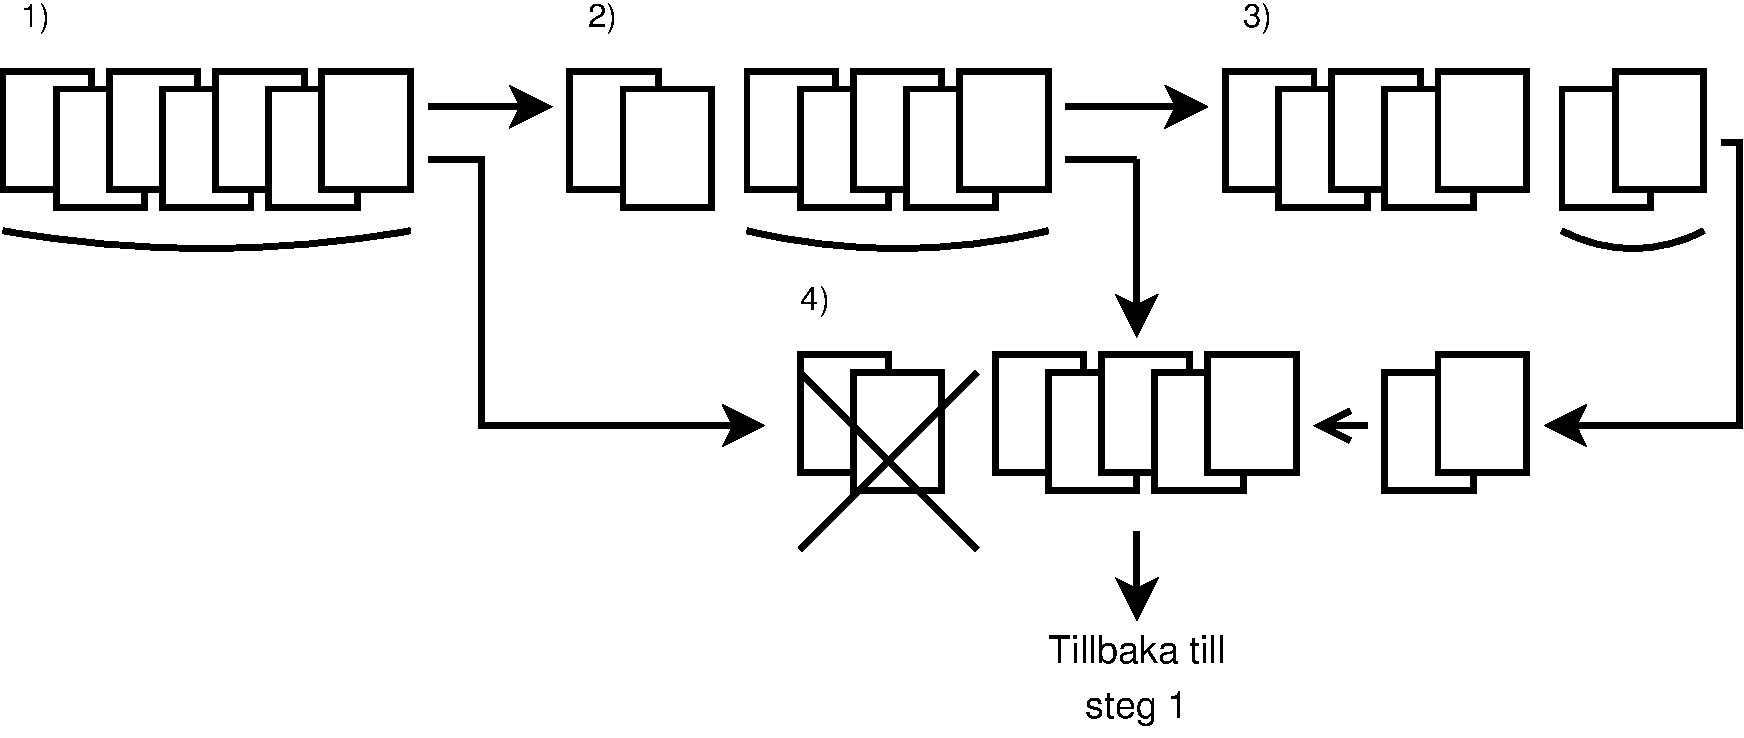
\includegraphics[width=0.95\textwidth]{bilder/HMM_flowchart}
  \caption{\notes{FÖRKLARANDE TEXT}}
  \label{fig:hmm-flowchart}
\end{figure}
 
Programmet initieras

(BILD)

Då programmet körts mer än x antal frames

(BILD)

klassificeringen sker lämpligen med en threshold 
De längsta sekvenserna går först


Antal tillstånd för modellen lika många som gesten den modellerar har symboler.
HMMs för statiska gester tränas för att känna igen sekvenser av samma symbol.
Med tränade modeller undersöker man sedan sannolikheten att en symbolföljd genererades av en viss modell.
Bäst modell vinner.

 \end{document}

